\section{Event Kinematics and Timing}
\label{sec:event_timing}
The kinematics of the underlying event effect the production and arrival times of the Cherenkov and scintillation light. In both 0\nbb and 2\nbb near the endpoint, the two electrons are produced most likely back-to-back with equal energy. These are distributions as shown in Fig.~\ref{fig:Kinematics} for \Te(Q=2.526~MeV). This is a good isotope choice due to the high natural abundance XX , however isotopes with higher endpoints such as Cd, Se, Ca would increase both the number of Cherenkov and scintillation photons improving the direction reconstruction and the energy resolution at the endpoint.

\begin{figure*}[ht]
  \centering
  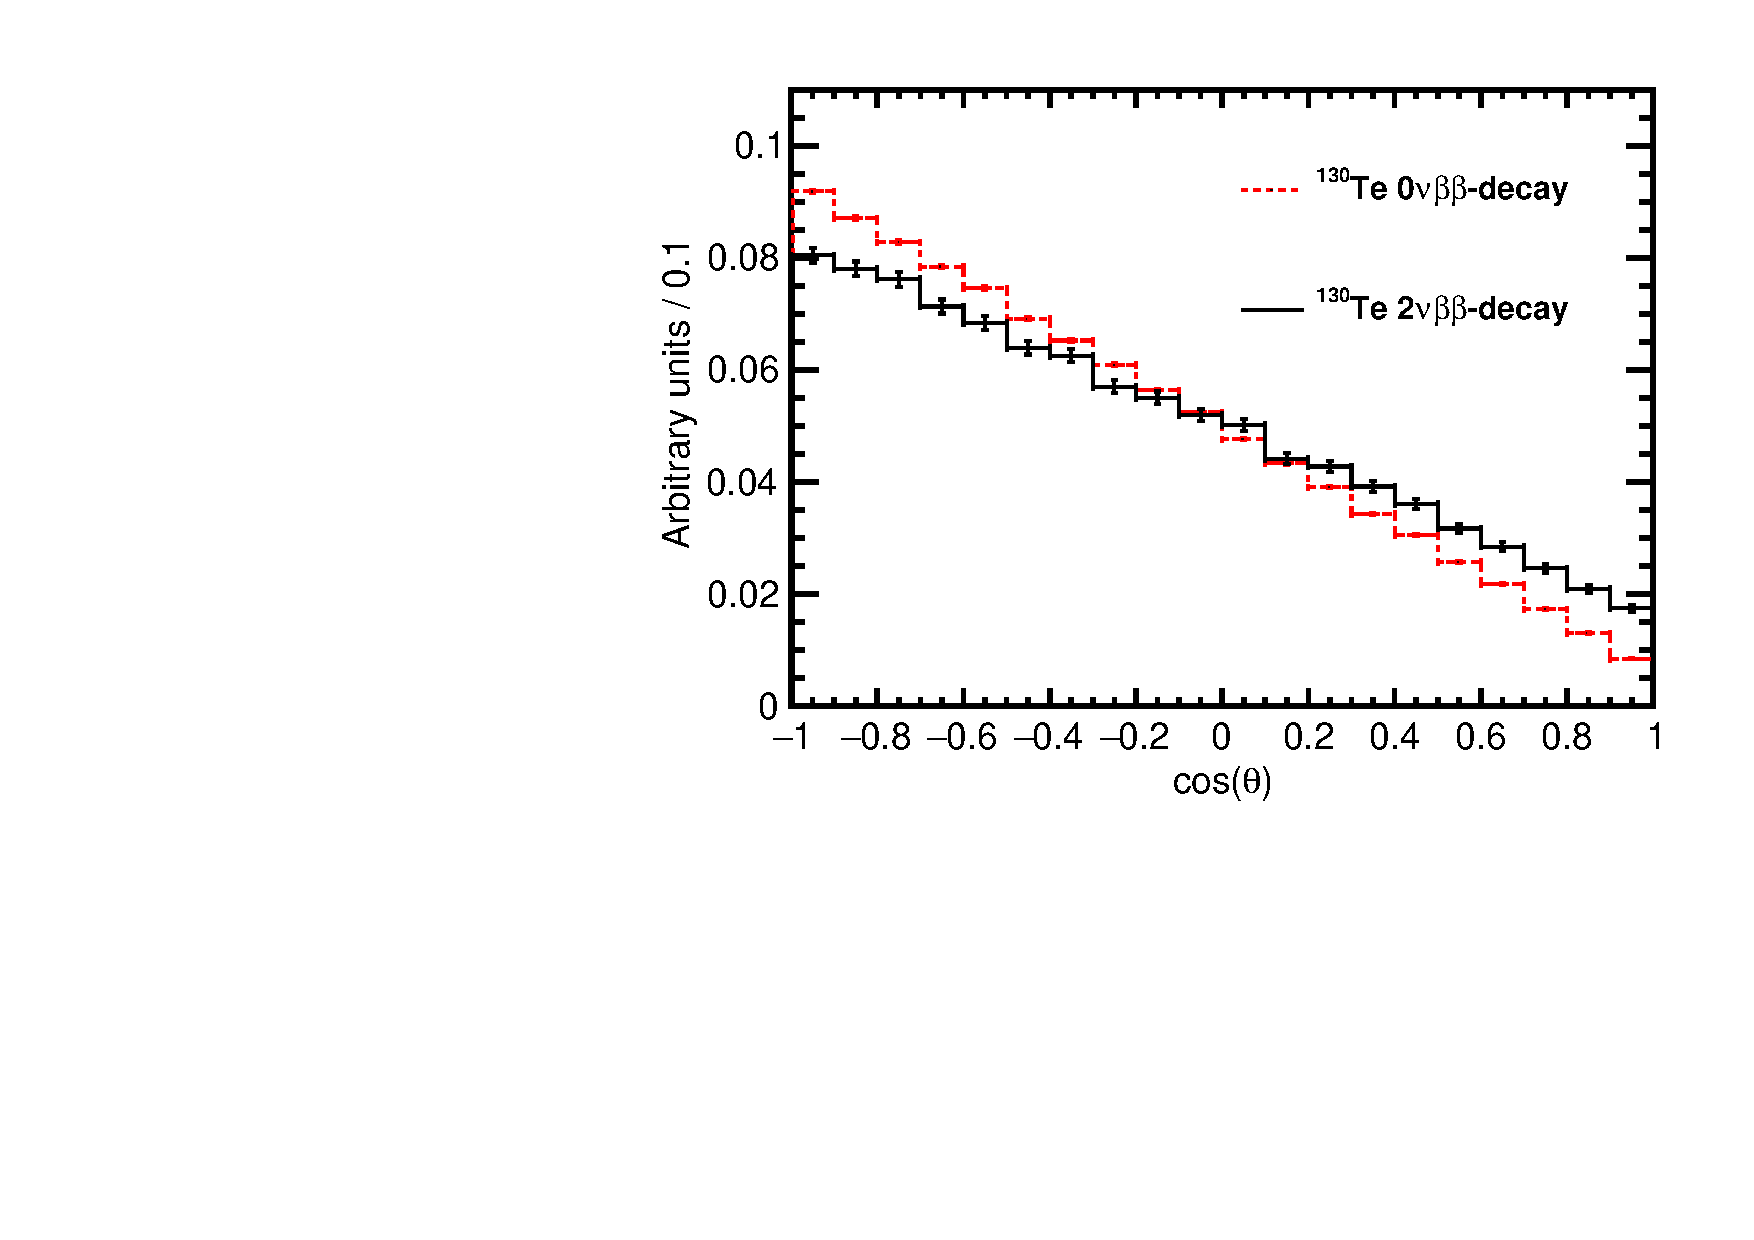
\includegraphics[width=0.49\textwidth]{hCos_Te130.pdf}
  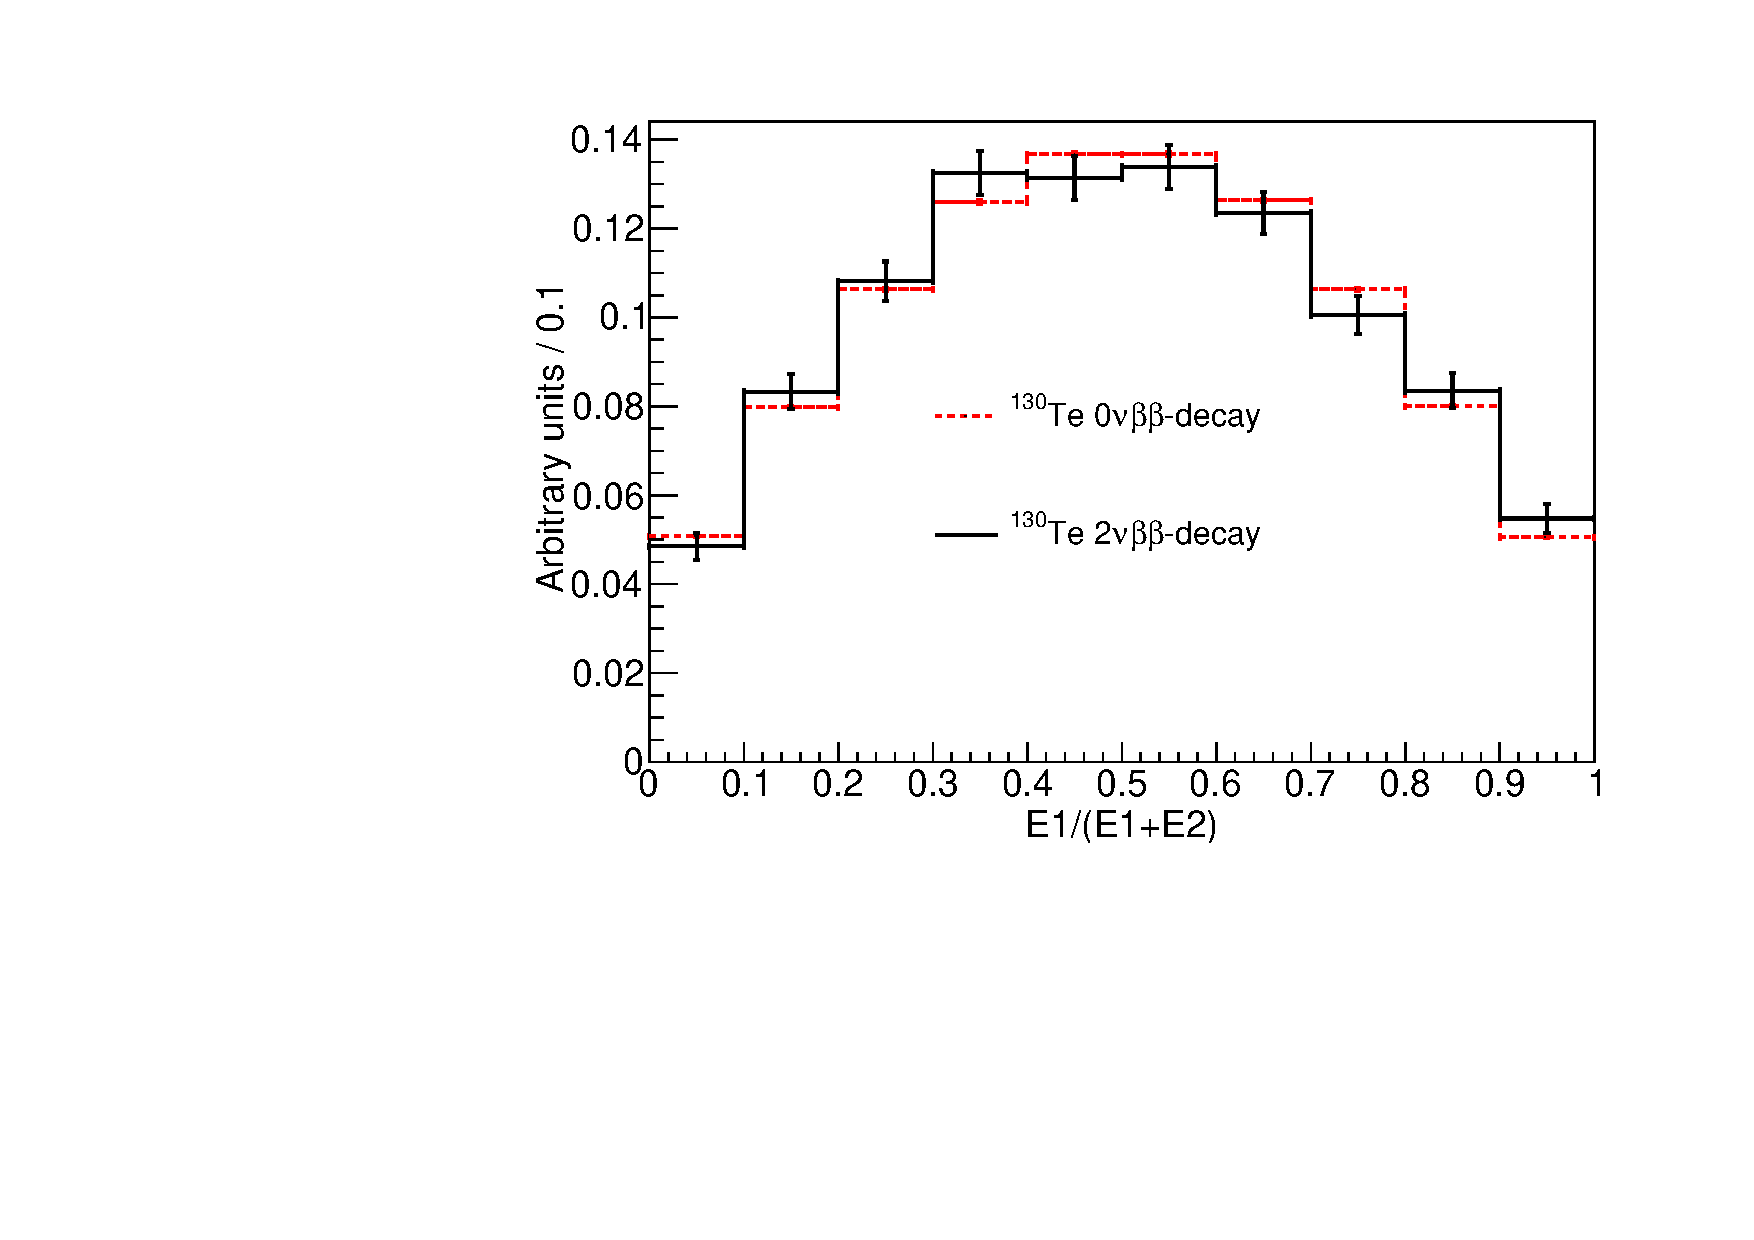
\includegraphics[width=0.49\textwidth]{hE1toQ_Te130.pdf}
  \caption{Comparison between kinematics of 0{\nbb} (\emph{dashed red
      lines}) and 2{\nbb} decays (\emph{solid black lines}) for events
    with the total kinetic energy of the electrons above 90\% of the
    Q-value. \emph{Left:} Cosine of the angle between two
    electrons. \emph{Right:} Fraction of energy carried by one of the
    two electrons. Due to limited statistic around the energy spectrum
    end point for 2{\nbb} decay we show statistical errors for each
    bin.}
  \label{fig:Kinematics}
\end{figure*}


%Should we recalculate for 130Te.
Examining the kinematics for one of the \bb electrons , a 1.4~MeV electron travels a total path length of 0.8~cm, has a distance from the origin of 0.6~cm in 0.030$\pm$0.004~ns  and takes 0.028$\pm$0.004~ns to drop below Cherenkov threshold. We note that due to scattering of the electron, the final direction of the electron before it stops does not correspond to the initial direction; however the scattering angle is small while the majority of Cherenkov light is produced. The Cherenkov light thus still encodes the direction of the primary electron. The scattering physics is handled by Geant4's ``Multiple Scattering" process which is valid down to 1~keV, where atomic shell structure becomes important\cite{geant4scatt}. Figures~\ref{fig:ArrivalTimeDist} and~\ref{fig:NPhotDist} show the output of the detector simulation for 1000 simulated \Te \vbb-decay events. The left panel in Fig.~\ref{fig:ArrivalTimeDist} compares PE arrival time between Cherenkov and scintillation light  and the right panel in Fig.~\ref{fig:ArrivalTimeDist} zooms in on the Cherenkov photon distribution which is key to direction and topographical reconstruction.

\begin{figure*}[ht]
  \centering
  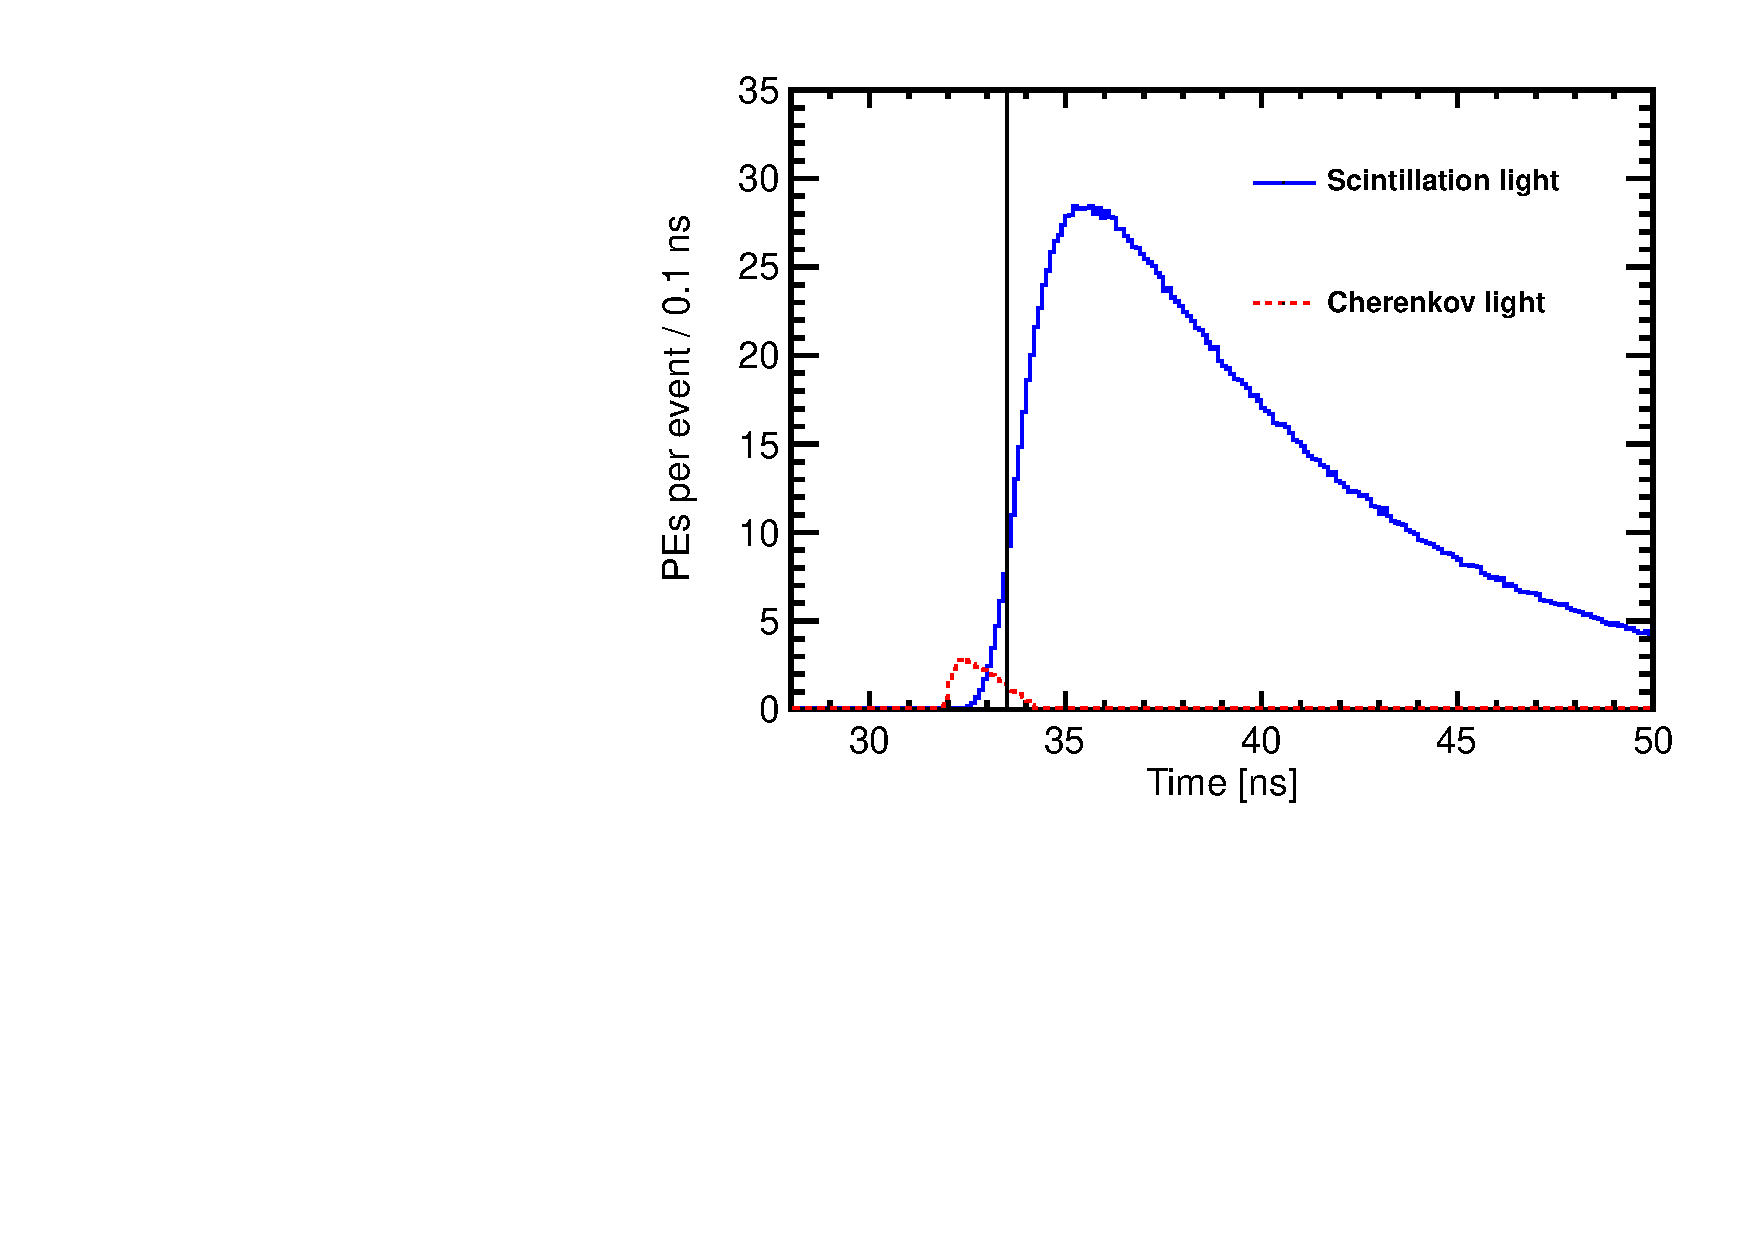
\includegraphics[width=0.45\textwidth]{hT_Te130.pdf}
  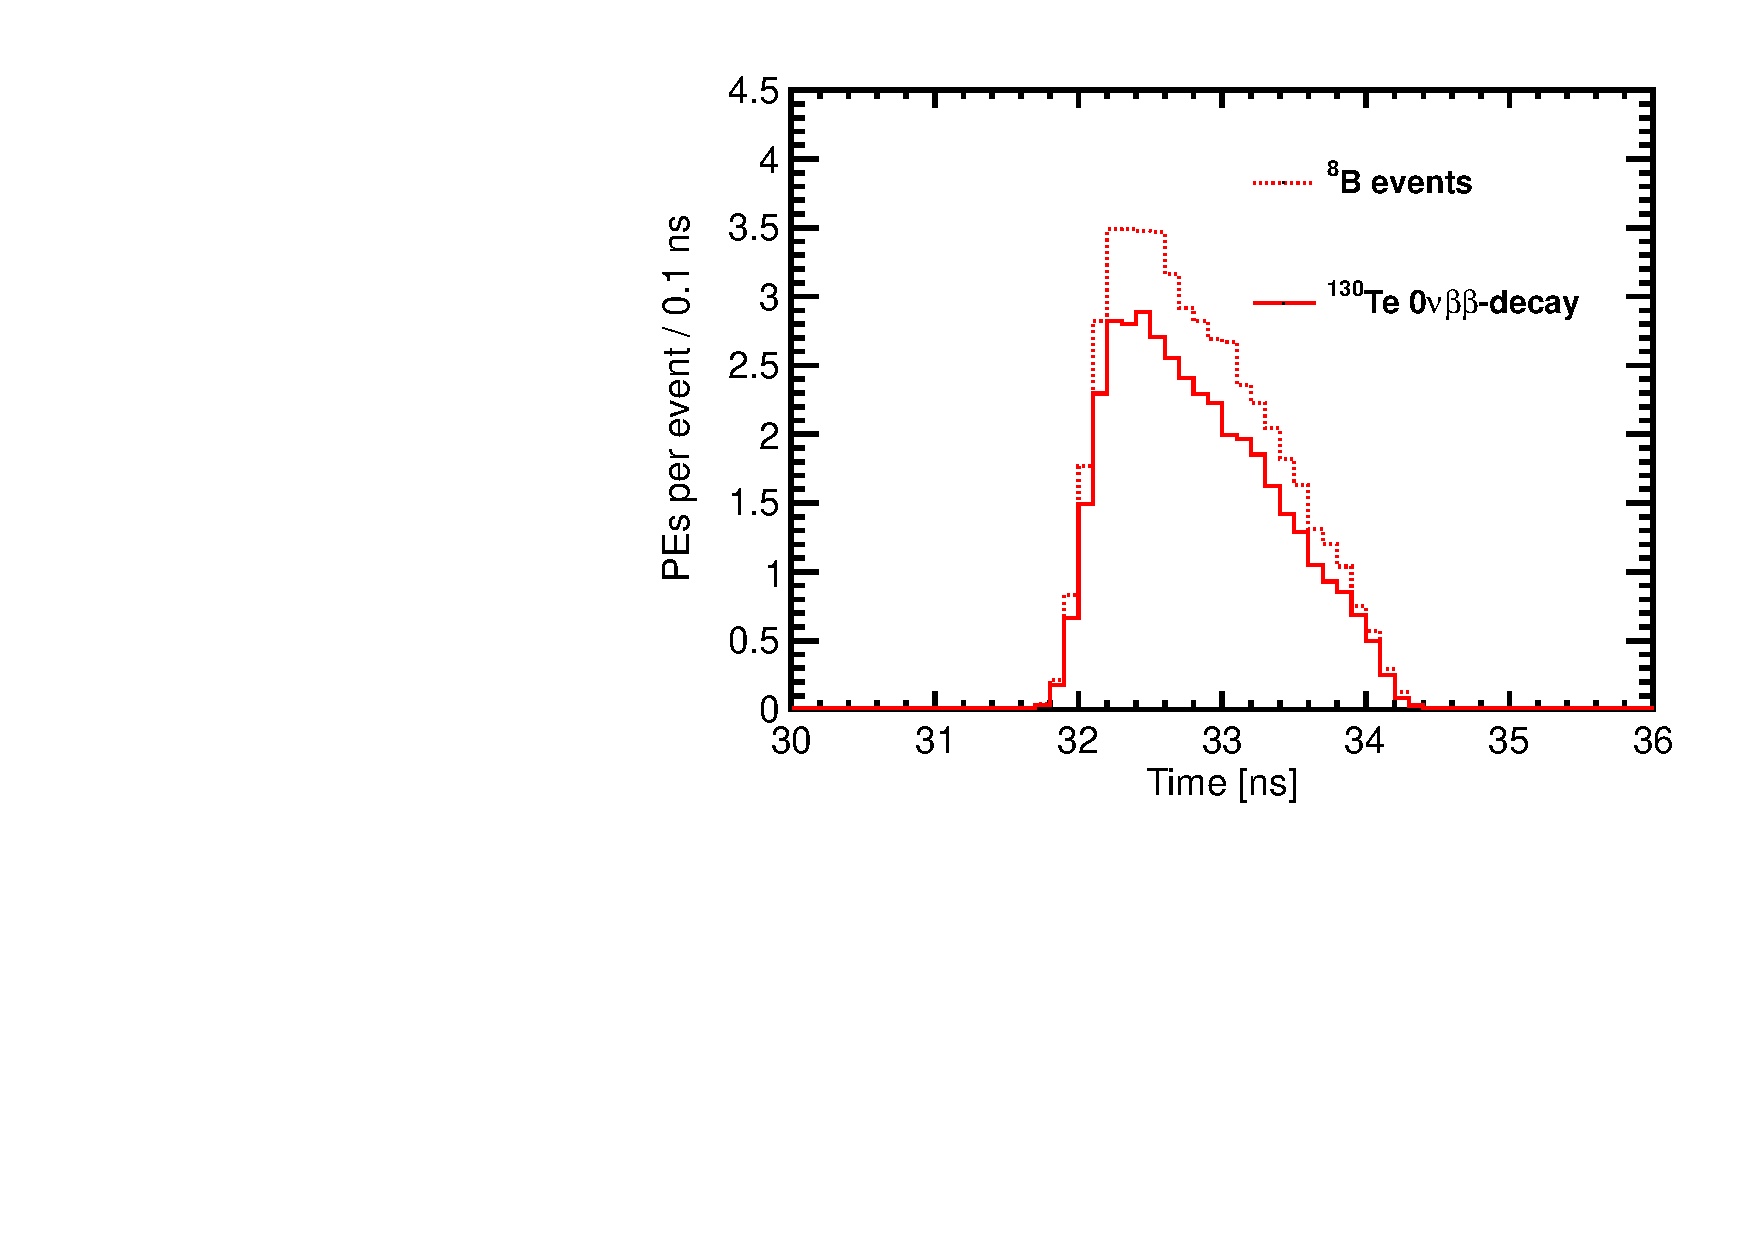
\includegraphics[width=0.45\textwidth]{hTche_Te130_B8.pdf}
  \caption{\emph{Left:} Photo-electron (PE) arrival times after
    application of the photo-detector transit time spread (TTS) of
    100~ps for the simulation of 1000 0{\nbb} decay events of
    $^{130}$Te at the center of the detector. PEs from Cherenkov light
    (\emph{dashed red line}) and scintillation light (\emph{solid blue
      line}) are compared. The black vertical line illustrates a time
    cut at 33.5 ns. \emph{Right:} Comparison between Cherenkov PEs
    arrival time for $^{130}$Te {0\nbb} decay (\emph{solid line}) and
    $^{8}$B (\emph{dotted line}) events. {\bf Distributions of the
      scintillation PEs arrival time are indistinguishable between
      $^{130}$Te 0{\nbb} decay and $^8$B due to identical total energy
      in the event, $Q(^{130}{\rm Te})=2.526$~MeV.} }
\label{fig:ArrivalTimeDist}
\end{figure*}

The scattering of \B solar neutrinos produces one electron with the same kinetic energy of the two electrons from the \bb-decay. The scintillation spectrum is unchanged since the electron's path lengths at these energies are too short to affect the effective vertex of the scintillation lighter. The number of Cherenkov photons is increased due to the increased electron kinetic energy but this alone is not sufficient to distinguish these event types. However, it may provide an extra handle on signal-background separation in combination (e.g. by using multivariative techniques) with other event parameters.

The positron decay of \C to the excited state of $^{10}$B produces gamma-rays from the annihilation of the positron and the de-excitation of the $^{10}$B nucleus. The gamma-rays travel several cm before depositing their energy. This leads to a more diffuse effective vertex and a smearing of the scintillation emission arrival times. This may be an effective way in the reduction of the \C background. The total number of Cherenkov photons is comparable to that from \nbb.

As shown in Fig.~\ref{fig:ArrivalTimeDist}, a time cut of 33.5~ns on the PE arrival time selects a sample of early PEs that includes the majority of Cherenkov photons. Scintillation PEs also are selected with this time cut. Figure~\ref{fig:NPhotDist} shows the total number of scintillation and Cherenkov PE per event for $\vbb$ signal and \B background events. 

\begin{figure*}[ht]
  \centering
  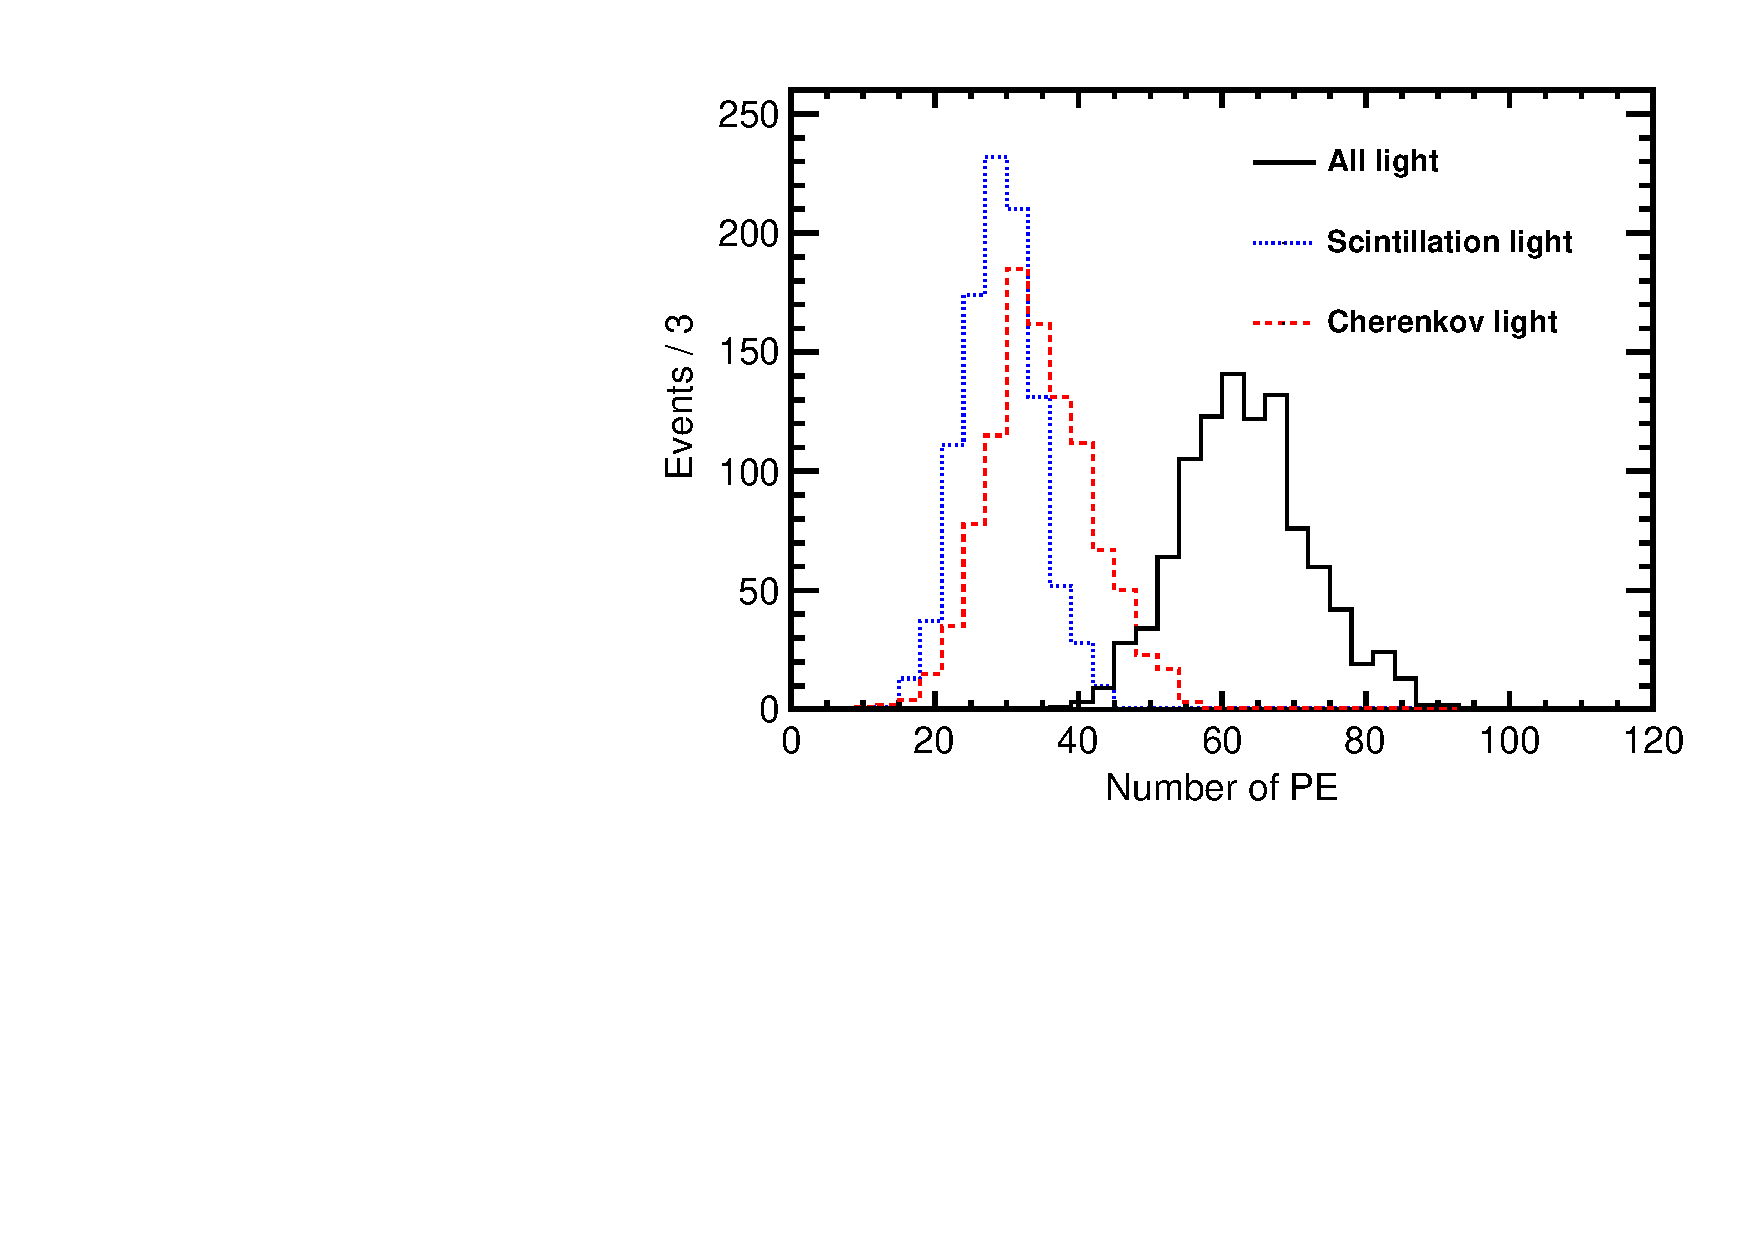
\includegraphics[width=0.45\textwidth]{hMomNPhot_Te130.pdf}
  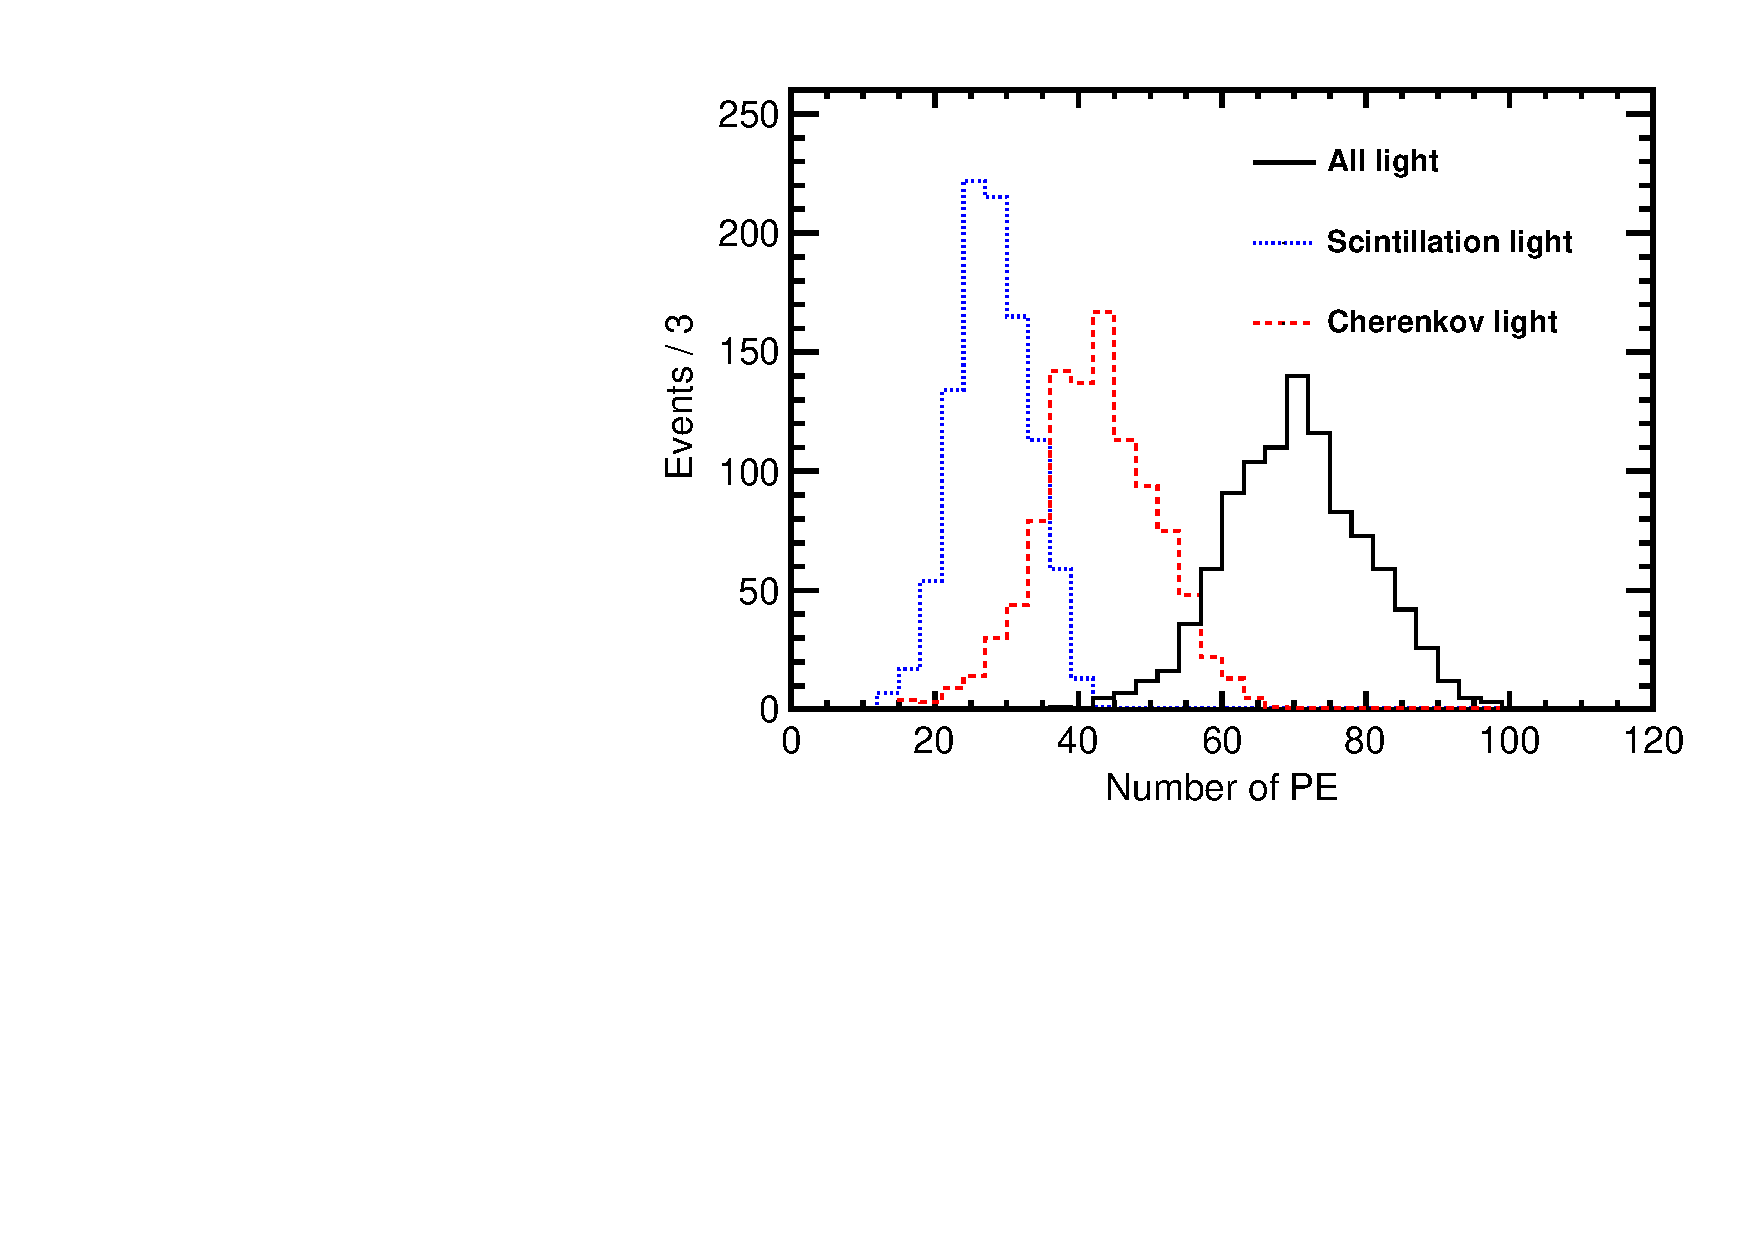
\includegraphics[width=0.45\textwidth]{hMomNPhot_1el_2p529MeV.pdf}
  \caption{Number of Cherenkov (\emph{dashed red line}), scintillation
    (\emph{dotted blue line}), and total (\emph{solid black line}) PEs
    for the simulation of 1000 $^{130}$Te 0{\nbb} decay (left panel)
    and $^8$B (\emph{right panel}) events.}
\label{fig:NPhotDist}
\end{figure*}

\textbf{FIXME: Does Andrey have the distance the gamma rays travel?} \\
\textbf{FIXME: Check on references from Inverse Beta decay for positron annihilation and info from KL meeting}\\
\textbf{FIXME: Do the early light plots add anything here, move this discussion?}\\

